\chapter{Computational Biology Background}
\label{c:background}

% \note{Roughly 25 pages ..?} 

This chapter provides the background knowledge necessary to understand the basic principles of mass-spectrometry-based analysis as applied to large-scale untargeted biological studies. A particular emphasis is given to the application of mass spectrometry techniques to the field of metabolomics. For a further reading on mass spectrometry, the reader is directed to a more comprehensive textbooks such as \cite{Hoffmann2007} and \cite{gross2006mass}. Reviews on the necessary data pre-processing steps of mass spectrometry data can be found for e.g. in proteomics \cite{Megger2013, Sandin2014, Smith2014} and metabolomic \cite{Castillo2011,Manuscript2013,Gika2014}.

\section{Computational Biology}

Since the discovery of the deoxyribonucleic acid (DNA) as the basic storage of genetic information, the same fundamental principle is found to govern the transmission of hereditary information common to all life on Earth. Following the central dogma of molecular biology:
\begin{center}\framebox{\textbf{DNA is transcribed into RNA, which is translated into proteins.}}\end{center}
In the central dogma, genetic materials are coded in the DNA, a strand of which consists of a series of nucleotides. The backbone of a nucleotide comprises sugar and phosphate groups attached to one of the four nitrogenous bases of \textbf{A}denine, \textbf{T}hymine, \textbf{G}uanine, and \textbf{C}ytosine, forming the four well-known alphabets of the DNA. The start of the transcription process begins with the unwounding of the double strand of the DNA into single strands. The single DNA strand is transcribed by a protein complex (RNA polymerase) into messenger ribonucleic acid (RNA), which can be be thought as nearly identical to DNA, with the crucial difference that the base \textbf{U}racil is used in place of thymine. The substitution of thymine to uracil allows RNA to perform its important function as the messenger RNA, which as the name suggests is the intermediate mechanism of messaging for the information contained in the chemically inert DNA. Messenger RNA is read by the ribosome, a part of the translational apparatus of the cell, and translated into amino acids, which are the building blocks of proteins. 

Since its initial proposal, this simple central dogma model has been challenged and expanded to acknowledge other factors that can influence the transcription and translation processes. Nevertheless, the central dogma serves to illustrate the flow of genetic information in a biological system. Different sub-fields of computational biology predominantly study the different entities and processes involved in the central dogma. Genomics is concerned with the large-scale study of the genome (the entire DNA in the organism) and how the genes encoded in the genome interact with each other. Sequencing technologies, in particular next-generation sequencing (NGS) machines such as Illumina and Ion Torrent, have been instrumental in revolutionising genomics by making possible the high-throughput and rapid sequencing of the entire DNA sequence from a sample \cite{metzker2010sequencing}. Transcriptomics focuses on understanding the transcriptome (the complete set of messenger RNA) and their measurement. Transcriptome relies on DNA micro-array technologies and more recently, have been increasingly performed by NGS sequencing as well. Proteins and their large-scale identifications and quantifications are studied in proteomics, while the complete set metabolites present in the sample and their expressions are the focus of metabolomics. Each successive layer of the -omics hierarchy, which comes closer to the actual physical expression of observable traits (phenotypes), introduces more complexity due to the increased number of ways of putting the building blocks in that layer together (Figure~\ref{fig:01}).

\todo[inline]{Draw this}
\begin{figure}[!tph]%figure1
\noindent \begin{centering}
\fboxsep=0pt\colorbox{gray}{\begin{minipage}[t]{235pt} \vbox to 100pt{\vfill\hbox to
235pt{\hfill\fontsize{24pt}{24pt}\selectfont TODO\hfill}\vfill}
\end{minipage}}
%\centerline{\includegraphics{fig01.eps}}
\par\end{centering}
\caption{The building blocks of the genome are the DNA nucleotides. In the transcriptome, the building blocks are the nitrogenous bases that comprise the RNA. In proteomics, the 20 amino acids residues make up the polypeptide comprising a protein molecule. In contrast, the building blocks of metabolites are the atoms (usually CHNOPS: carbon, hydrogen, nitrogen, oxygen, phospor and sulphur) that comprise a large range of compounds, such as lipids, amino acids, vitamins, etc., with varying physical and chemical properties}\label{fig:01}
\end{figure}

\section{Mass spectrometry-based omics\label{sub:omics}}

The two -omics closest to the phenotype in Figure~\ref{fig:01} rely on mass spectrometry, usually coupled to a separation intrument such as chromatography, to perform measurements and quantification of the biological entities of interest. Proteomics and metabolomics are briefly expanded in this section, while details on the set-up of the instruments can be found in Section~\ref{sub:mass-spec}.

Proteins, considered the building blocks of life, serve critical roles in an organism by performing cellular maintenance, catalysing chemical reactions, carrying molecules across cell membranes and many other essential functions. The primary building blocks of a protein are amino acids, which results from the translation of messenger RNA. An amino acid consists of the amine group (-NH$_2$), a carboxylic group (-COOH) and a side chain. Through the loss of water molecule, amino acids can be chained to each other through the peptide bonds, collectively forming a peptide. Each amino acid can be described by a unique letter drawn from a set of 20 chemical alphabets, and consequently a peptide can be succinctly described as a string of letters corresponding to its constituent amino acids. While the sequence of amino acids comprising a protein is largely coded by genes in the genome, this process is far from deterministic. In a process called post-translational modification \cite{mann2003proteomic}, proteins can be chemically modified after synthesis in a way that completely alters its structure and folding stability, e.g. through phosphorylation, methylation or glycosylation. This results in a large variety of protein diversity present in the biological system, and it is the large-scale characterisation of identities and quantities of proteins that is of particular interest to \textbf{proteomics}. 

Apart from proteins, numerous other chemical reactions essential for sustaining life also happen inside a cell. In catabolic reactions, large organic molecules  within a cell are broken into energy and smaller molecules. These serve as the input to anabolic reactions, producing the basic building blocks of a cell such as proteins and nucleic acids. Both anabolic and catabolic reactions are usually catalysed by enzymes, and together these two reactions comprise the metabolism of an organism. Metabolites are the molecules involved during or produced as the by-products of metabolism. Through the help of various enzymes, metabolites are transformed from one form to another in a series of chemical reactions as part of the metabolic pathways. Some examples of common metabolites are the various amino acids, fatty acids, and vitamins (e.g. B3 and B12) and minerals (e.g. phosphorus, iron and zinc). The overall set of metabolites that can be found within an organism is collectively called the metabolome. \textbf{Metabolomics} studies the metabolome on a large scale, usually for the purpose of identifying and quantifying their differences in the particular organisms or tissues under various experimental or physiological conditions. As metabolomics as a study is considered to be the closest to the phenotype, changes to the metabolome often result in physically observed properties, and indeed changes in the metabolite composition of an organism may be caused by responses to environmental and genetic factors \cite{Katajamaa2007}. Studying the metabolome provides us with an instantaneous 'snapshot' of the chemical activities that are occurring in the cell at that moment. 

\section{Mass Spectrometry\label{sub:mass-spec}}

Atoms are small building blocks of matter. An atom has a nucleus at the centre, which consists of positively charged protons and neutrons with no charge. Electrons, having negative charge, are bound to the neucleus through electromagnetic force. The overall charge of the atom is therefore determined by the number of electrons and protons that it has. The atom is called a positive ion when there are more protons than electron, otherwise it is a negative ion. Two or more atoms hold together via chemical bonds comprise a compound. The molecular mass of a compound is the sum of the molecular mass of its elements, measured in Dalton (Da), where one Da is $\frac{1}{12}$ of the molecular mass of the carbon element ($^{12}C$). Elements in nature occur as isotopes. Isotopes are naturally occurring elements that have the same number of protons (same atomic number) but different number of neutrons (different molecular masses). Each elements has many isotope species, for instance carbon has two isotopes: $^{12}C$ with molecular mass 12.000000 at 98.890\% abundance in nature, and $^{13}C$ with molecular mass 13.003355 and 1.110\% abundance. The term `mono-isotopic' refers to the most abundant isotope species of an element. The exact mass of a compound can therefore be calculated from the formula sum of the masses of its constituent mono-isotopes. The nominal mass of a compound is similarly calculated by summing the integer masses of the constituent mono-isotopes (e.g. the nominal mass of $H_2O=1+1+16=18$).

Mass spectrometer (MS) coupled to liquid chromatography, forming the set-up of liquid chromatography mass spectrometry (LC-MS), is the preferred measurement platform for determining the elemental composition and the abundance of the analytes (proteins or metabolites) in proteomics or metabolomics studies. MS instruments can be ranked by the ascending order of their resolving powers of their mass analyser: \textbf{(1)} time-of-flight MS, \textbf{(2)} quadropole MS, and lastly \textbf{(3)} Fourier transform ion-cyclotron MS. A higher resolving power corresponds to a better ability of the instrument to detect small differences in mass-to-charge (m/z) ratios. Having a higher resolving power is generally very useful when trying to identify which metabolites are present in the sample. Modern high-precision MS instruments have very accurate resolving power, with accuracy up to several parts-per-million. The difference between the observed mass-to-charge value to the exact-mass-to-charge value of a compound is the mass accuracy of a mass spectrometry instrument, measured in parts-per-million, i.e. $\text{mass accuracy} = 1e6 * \frac{(\text{observed m/z} - \text{exact m/z})}{\text{exact m/z}}$. 

\subsection{Metabolomics\label{metabolomics}}

In recent years, the combination of liquid chromatography coupled to mass spectrometry (LC-MS) has emerged as one of the most widely used techniques in untargeted metabolomic studies. Metabolites in the extracted sample cannot be introduced at once as direct injection into MS due to ion supression effect \cite{Annesley2003}, where compounds 'compete' for charges during the ionisation process inside the MS. Due to this ion supression effect, metabolites present in low abundance might not be ionised and therefore not detected in the resulting mass spectra. As a result, it is necessary for metabolites to be separated before being introduced gradually into the inlet of the ionisation source. Separation techniques such as liquid chromatography LC coupled to MS is commonly used for this purpose. In liquid chromatography, the mobile solvent containing the analytes (metabolites) is introduced and pumped into the stationary phase of the chromatographic column. Metabolites elutes at different time through their interactions with the capillary, based on the hydrophobicity, charge and other chemical properties of the metabolites. The time it takes for these metabolites to elute through the stationary phase of the LC column is called the retention time (RT). LC-MS tends to be easier to automate and suitable for high throughput experiments. Sample preparations for an LC-MS set-up also tends to be simpler compared to the alternative of separation via gas chromatography, while compounds across a wide range of polarity can be separated \cite{Hoffmann2007}. 

Metabolites that elute from liquid chromatography are then vaporised and ionised inside the mass spectrometer. This is usually accomplished through soft-ionisation methods such as atmospheric pressure ionisation or electrospray ionisation (ESI). The distinction between soft- and hard- ionisation methods come from how 'soft' methods do not break the chemical bonds of the compound during the ionisation process, which stands in contrast to hard-ionisation methods, such as the electron impact ionisation, that breaks the chemical bonds in the neutral molecules of compounds. ESI can be directly coupled to LC, so often, it is the preferred method of ionisation. In ESI, the sample analyte is dissolved into a solvent and sprayed through an electrospray. It is the resulting charged aerosol that enters the vacuum of the mass spectrometer, generating charged molecular ions and their corresponding fragment ions. The generated ions are separated by the mass analyser inside the MS instrument according to their m/z (mass-to-charge) ratios and the detected signal abundance for a particular m/z value. The result of this process is a mass spectrum: a two dimensional representation of m/z values to signal intensities. The final raw data produced by an LC-MS setup is called the ion chromatograms: a collection of mass spectra over the range of elution time. The entire raw data can therefore be characterised by a set of vector of m/z, intensity and retention time, and for every slice on the ion chromatogram sharing the same RT value (a scan), a mass spectrum is produced from metabolites that elute at that same retention time. A mass spectrum is the observed m/z and intensity (abundance) values of the peaks that result from fragmentations of the metabolites during the scan. When the MS instrument is run on the full-scan mode, the entire m/z range is selected for fragmentation. 

\todo[inline]{Redraw this to be simpler.}
\begin{figure}[htb!]
\noindent \begin{centering}
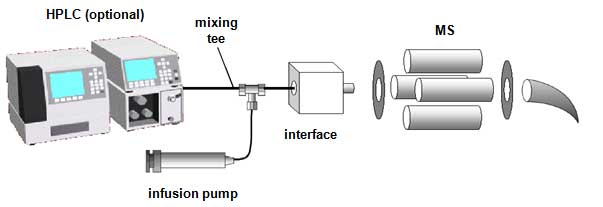
\includegraphics[width=0.8\textwidth]{02-background/figures/Fig-1}
\par\end{centering}
\caption{\label{fig:LC-MS-setup}A typical LC-MS set-up. High performance liquid chromatography instruments are used to separate metabolites (by their chemical properties) in the sample before they are gradually introduced into the mass spectrometer.}
\end{figure}

\todo[inline]{Redraw this to illustrate the point better.}
\begin{figure}[htb!]
\noindent \begin{centering}
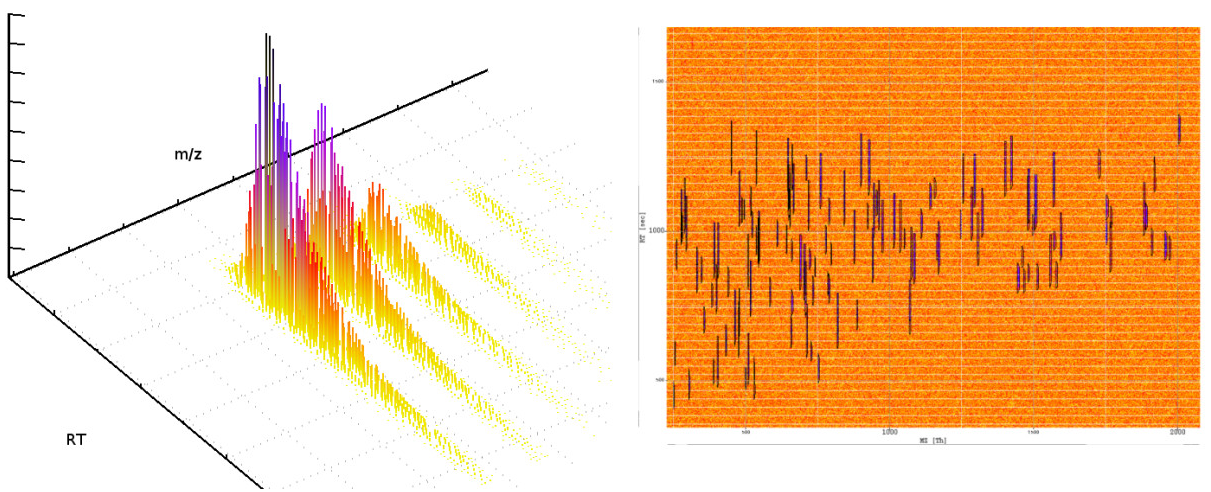
\includegraphics[width=0.75\textwidth]{02-background/figures/report_0001}
\par\end{centering}
\caption{\label{fig:LC-MS-data}The resulting raw data (ion chromatograms) produced from an LC-MS experiment. We can view the data as a 3D profile (left) and as a 2D profile seen from the top (right). A slice of the data on the m/z axis is the mass spectrum. Each mass spectrum is produced by a scan of the mass spectrometer. A collection of mass spectra is produced over the whole range of retention time. A point in the raw data is thus characterised by its intensity value on the m/z and retention time axes.}
\end{figure}

\subsection{Proteomics and Glyomics}

For mass spectrometry analysis of proteins, the samples to be analysed come either in the form of tissues or as body fluids, such as urine, plasma and serum. Different types of samples will demand the appropriate sample handling protocol in the sample preparation stage. Next, cells extracted from the sample are broken down, allowing proteins to be isolated from other constituent parts of the cell, for instance the DNA, lipids and other metabolites that are present. The purified proteins are then separated. Traditional 2-D gel electrophoresis method allows proteins to be separated according to their size (molecular mass) in one axis and according to their isoelectric points (the pH where the molecule carries no electrical charges) on another. Because 2D-GE approach is tedious and time-consuming, liquid chromatograph mass spectrometry has gotten more popular as the preferred separation technology as it enables the large-scale high-throughput separation of thousands of proteins in a single chromatographic run. Enzymes that can cut the peptide bonds, such as trypsin, are then used to digest proteins into shorter peptide fragments. Using certain enzymes, the cleavage of the peptide bonds happen at specific and predictable spots, allowing well-defined and easily identifiable peptide fragments to emerge. For instance by using trypsin as the digestion enzyme, the cleavage of the protein happens after each arginine or lysine amino acid is encountered, unless a proline amino acid comes next. An initial separation process (pre-factionation) can also be performed on the digested peptides using liquid chromatography, resulting in different fractions, which can then be ran separately through the hypenated set-up of LC-MS (Figure~\ref{fig:LC-MS-setup}) for mass fragmentation analysis in a manner similar to metabolomics analysis (described in the following paragraphs in Section~\ref{metabolomics}). This yields the peptide mass fingerprint, which although challenging, can generally be used to match the resulting peptide fingerprints against a database of reference fingerprints for identification of the peptides and correspondingly the entire protein. 

\subsection{Fragmentation\label{sub:fragmentation-background}}

Fragmentation through tandem MS or MS\textsuperscript{n} instruments can be used to provide further fragmentation information for metabolite identification. As suggested by its name, tandem MS requires two MS analysers operating in tandem. Ions resulting from the initial fragmentation of metabolites in the first MS analyser are selected for further fragmentation in the second MS analyser. The ions selected for the first MS analyser stage are called the precursor ions. In data-dependent acquisition (DDA), precursor ions within some small m/z windows are selected based on some predetermined rules (such as fragmenting the top few most intense precursor peaks in each scan). As a result, typically a small percentage, e.g. less than a fifth of all precursor peaks in the full-scan mode data are selected for MS-MS fragmentation \cite{Smith2004}. Peaks that are generated from the fragmentation of the precursor ions in the second MS stage are called product ions. Fragmentation spectra of product ions are often used as the unique `fingerprint' identifiers of the structural composition of the precursor ions. This is described further in Section~\ref{sub:identification}. An alternative to DDA is the data-independent acquisition (DIA), where no selection of precursor ions needs to be specified as all peaks within a defined m/z range are fragmented. DIA results in a more complex fragmentation spectra due to multiple peptides/metabolites being fragmented together in the same m/z window, and require sophisticated analysis strategy to deconvolve the signals from the noise. 

\section{Metabolomics Pipeline: From Raw Data to Biological Hypothesis}

The raw LC-MS data is noisy, so pre-processing has to take place before analysis can be performed and biological conclusion drawn. The raw LC-MS data has to go through successive pre-processing and transformations along the data pre-processing pipeline before it can be analysed. The main steps of LC-MS data preprocessing generally involve peak detection and the filtering of noise, the matching of identical peaks across samples (alignment), identifications of peaks and lastly, data normalization and visualization. \ref{fig:Preprocessing-pipeline-of} shows these key preprocessing steps in the typical LC-MS data processing pipeline, which is elaborated further next.

\todo[inline]{Redraw this to make it look nicer..?}
\begin{figure}[htb!]
\noindent \centering{}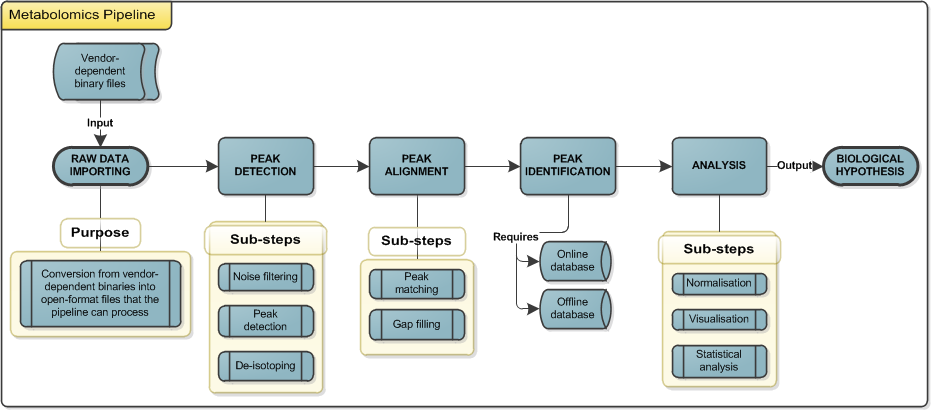
\includegraphics[width=1\textwidth]{02-background/figures/Drawing1}\caption{\label{fig:Preprocessing-pipeline-of}Preprocessing pipeline of LC-MS metabolomics data.}
\end{figure}

\subsection{Peak Detection\label{sub:related-peaks}}

The raw LC-MS data is imported into the pipeline. Beginning as a vendor-proprietary format, the raw data is converted into open XML-based format for storing mass spectrometry data, such as the mzXML or mzML format \cite{Pedrioli2004}. Noise filtering is performed as a preliminary filtering to remove noises and artifact signals due to the various chemical noises that also occur during the ionisation process. Peak detection is then performed to identify areas and intensities of peaks. A survey of the different approaches towards peak detection can be found in \cite{Zhang2009}, but what is important to note is at this stage, additional peaks can potentially be introduced due to peaks falsely detected from chemical noises, e.g. as a result of the contaminants present in the sample, while on the other hand, peaks that should be detected can instead be missing as a consequence of setting incorrect parameters for the detection step, e.g. by setting threshold values that are too low. 

Additionally, not all observed peaks would correspond to true precursor ions of the metabolites, since peaks could also be generated by other entities sharing the same identifying mass value, due to the presence of isotopes, contaminants, adducts and other signal artifacts in the sample (\cite{Keller2008}). In particular, due to the presence of naturally occurring isotopes (e.g. $^{13}C$) and the formation of adducts (the addition of a molecule ion to another), one precursor ion corresponding to a single metabolite alone can produce many observed peaks in the mass spectrum, forming a distribution of isotopic peaks at different m/z values but having similar chromatographic peak shapes in their elution time profiles. As one of the main challenges of peak detection comes from the presence of these isotope peaks, the de-isotoping step is often performed as an integral part of the peak detection step. The presence of multiple peaks that can be traced back to a single metabolite \todo{Write more about related peaks stuff.}

\subsection{Peak Alignment\label{sub:alignment-tools}}

The next step in the LC-MS data processing pipeline is the peak alignment step, where peaks from different LC-MS runs have to be matched. Experiments in biology usually involve the comparison of multiple samples. Samples can be produced as either biological or technical replicates. Biological replicates are obtained from the same organism studied under varying conditions. The organism studied are usually exposed to different factors (e.g. treatment or no treatment) controlled throughout the course of the experiment. Biological replicates are necessary to determine entities that are differentially expressed across samples. In contrast, technical replicates are obtained from the same samples analysed multiple times. Technical replicates are necessary to account for variability and measurement errors throughout the experiment. Since experiments in biology usually involve a comparison of multiple samples, it is necessary to align the LC-MS data produced from multiple samples in order to compare them. Alignment methods attempt to match peaks in correspondence across replicates. 

An initial approach towards alignment of replicates would be to spike a known amount of internal standards into each sample before running them through the LC-MS instruments. The peaks generated from the standards can be used as 'landmark' peaks to linearly shift the retention time in each sample, usually against a reference sample. Alternatively, labelling experiment can also be done by chemically labelling metabolites in two samples with isotopic reagents. The samples are then mixed before the LC-MS experiment and run through a single LC-MS run. The same metabolites from two samples would generally appear at close retention time, making alignment easy. However, labelled experiments consume expensive reagents, are more difficult to prepare and harder to compare across laboratories and to various mass spectral databases online for identification. Consequently, it is common for LC-MS experiments to be performed label-free without relying on such labelling information. This is called label-free experiments. To be comparable, the results from these label-free experiments need to be aligned, using peak alignment methods.

Broadly speaking, the main challenge in the peak alignment stage of label-free experiments is caused by the poor reproducibility of retention time, with potentially large non-linear shifts and distortions across LC-MS runs produced from different analytical platforms. Consequently, most alignment methods correct for those shifts and distortions by finding -- either explicitly or implicitly -- a mapping function $f$ that maps time $t$ in one replicate to $f(t)$ in another. The mapping function $f$ should be a monotonically smooth and increasing function, since elution orders of peaks that come out from the liquid chromatography instrument are generally preserved across replicates, at least for the data produced from the same LC-MS instruments. Alignment methods can therefore be broadly divided into two categories: warping and direct matching methods \cite{Smith2013}. Warping methods perform RT correction of peak features before establishing their correspondences across replicates. Warping methods attempt to correct the RT drifts present across runs, by fitting an RT correction function (typically a regression model), using either the full LC-MS profile data or the peak feature data alone. Early warping approaches, such as dynamic time warping \cite{Sakoe1978}, correlation optimised warping \cite{Nielsen1998} and parametric time warping \cite{Eilers2004}, are predominantly based on dynamic programming, and use only the time information present in the Total Ion Chromatogram, although more recent warping approaches have started to consider the m/z dimension as well \cite{Christin2008}. Once the time warping resulting in RT shifts have been corrected, the correspondence of peaks can be found through any method that matches peak features across runs. 

The alternative approach towards alignment is the direct-matching methods, where the warping step is skipped and peak features are directly matched across replicates to establish their correspondences. Direct approaches therefore require that the peak (i.e.\ feature) extraction step has already been completed. Direct matching methods can be preferred in certain cases due to their simplicity, while still offering good performance \cite{Lange2008}. The majority of direct matching approaches consist of two stages: computing feature similarity and using this similarity to match the features. A wide range of feature similarity measures have been proposed to compare the m/z and RT values of two peaks, including normalised weighted absolute difference \cite{Pluskal2010}, cosine similarity \cite{Hoffmann2012a}, Euclidean distance \cite{Ballardini2011}, and Mahalanobis distance \cite{Voss2011a}. Once similarity has been computed, feature matching can be established through either a greedy or combinatorial matching method. 

Many approaches have been proposed for direct matching of peak features. Greedy direct-matching methods work by making a locally optimal choice at each step, in the hope that this will lead to an acceptable matching solution in the end. RTAlign in MSFACTs \cite{Duran2003} merges all runs and greedily groups features into aligned peaksets within a user-defined RT tolerance. Join Aligner \cite{Pluskal2010} in MZmine2 merges successive runs to a master peaklist by matching features greedily according to their similarity scores within user-defined m/z and RT windows. Similarly, MassUntangler \cite{Ballardini2011} performs nearest-distance matching of features, followed by various intermediate filtering and conflict-resolutions steps. Recent advances in direct matching methods have also posed the matching task as a combinatorial optimisation problem. Simultaneous Multiple Alignment (SIMA) \cite{Voss2011a} uses the Gale-Shapley algorithm to find a stable matching in the bipartite graph produced by joining peaks (nodes) from one run with peaks from another run that are within certain m/z and RT tolerances. \cite{Wang2013} explores the application of the classical Hungarian algorithm to find the maximum weighted bipartite matching. BIPACE \cite{Hoffmann2012a} establishes correspondence by finding the maximal cliques in the graph. SMFM \cite{Lin2013} uses dynamic programming to compute a maximum bipartite matching under a relaxed bijective mapping assumption for time mapping.

Alignment methods can also be categorised depending on whether they require a user-defined reference run to be specified. When such reference is necessary, the full alignment of multiple runs is constructed through successive merging of pairwise runs towards the reference run (e.g. MZmine2's Join aligner in \cite{Pluskal2010}. Alternatively, methods that do not require a reference run can either operate in a hierarchical fashion -- where the final multiple alignment results are constructed in a greedy manner by merging of successive pairwise results following a guide tree (e.g. SIMA, described in \cite{Voss2011a}) -- or by pooling features across runs and grouping similar peaks in the combined input simultaneously (e.g. the \textit{group()} function of XCMS in \cite{Smith2006}).

Label-free experiments pose many challenges in analysing replicates from different LC-MS runs. In particular, peaks from different runs can experience a potentially non-linear shift in retention time across chromatograms \cite{Podwojski2009}. There is often a large amount of variations in the retention times across the replicates. Retention time variation could be due to instrument-specific factors (the condition of the chromatographic column itself. including flow rate variations, gradient slope and temperature \cite{Christin2008}) or experiment-specific factors (e.g. instrument malfunctions or columns that need be replaced mid-experiment). Both factors are difficult to control, even in a careful experimental setting. Consequently, a single peak from one replicate can have several potential matches peaks in another replicate, whilst having no matches in another replicate. This is exacerbated by the uncertainties introduced due to parameter selections in the preceding steps of the pipeline. As a result, replicates produced by different LC-MS platforms or from different laboratories cannot be easily aligned to each other. In particular, the non-linear variation in retention time makes aligning technical replicates (which contains the same composition of metabolites) difficult and aligning biological replicates (which may not contain the same composition of metabolites) even more challenging. Since large-scale untargeted metabolomics study can generate a huge number of samples (see \cite{DeVos2007a,Creek2011}), having a reliable and accurate peak alignment step during data preprocessing is important. Peaks that are improperly aligned can lead to false positives, and especially for untargeted label-free metabolomic experiments, the presence of even relatively small errors in any steps preceding the identification stage (including alignment) can result in significant differences to the final analysis and biological conclusions \cite{Chawade2015}. Errors or uncertainties inadvertently produced in any sub-step before identification would be carried forward forward in the pipeline. Improper preprocessing steps can also introduce variabilities that obscure important biological variations of metabolites themselves. 

\subsection{Peak Identification\label{sub:identification-background}}

The problem of identification of LC-MS data from peptides is referred to as peptide mass fingerprinting. As proteins are cleaved into peptides that are unique, the resulting fragmentation spectra are also expected to be unique to a protein. The theoretical peptide spectra can then matched against a reference spectra library. In practice, the resulting fragmentation spectra are not entirely unique and multiple hits can be returned from the spectra library, particularly in the case of libraries that have a large number of records. Identification is more difficult for metabolites due to the inherent complexity in metabolomics samples. A complete characterisation of the entire metabolome of any species is very difficult (for instance the human plasma and serum metabolome is still not fully characterised \cite{dunn2011procedures}). 

Untargeted identification Metabolite identification is challenging in untargeted metabolomic studies due to the vast number of metabolites present in sample and the diversity in elements that comprise a metabolite. Unlike the genome that has four nucleotide bases as its sole alphabets, or proteins with twenty one amino acids as their building blocks, metabolites are harder to characterise structurally. The basic building blocks of a metabolite are atoms (commonly CHNOPS) that can be arranged in a variety of configurations in a single molecule alone. Similar to proteomics, the primary metabolite identification techniques relies on matching the accurate mass information of compounds to the set of chemical alternatives in a mass spectral database. The goals of the identification process are to distinguish between (in increasing levels of difficulty): \textbf{(1)} metabolites with different nominal masses, \textbf{(2)} metabolites with the same nominal masses, but different formula and monoisotopic masses, and finally \textbf{(3)} metabolites with the same nominal and monoisotopic masses, but different chemical structures (including chirals and isomers, such as leucine and isoleucine) \cite{Dunn2012}.

Having a high mass accuracy is crucial here as it reduces the size of possible alternatives. However, even at the very high mass accuracy of 1 ppm, the number of possible formulae matched by accurate mass is still too large to allow for definite metabolite identifications \cite{Kind2006}. Identification is particularly difficult for metabolites present in low abundance in the samples. Consequently, widely-used metabolomics analysis tools like mzMine \cite{Pluskal2010} employ sophisticated heuristics (such as the Seven Golden Rules) to narrow the formulae space based on various chemical constraints. Additional information such as the isotope patterns of compounds, and their fragmentation patterns (obtained from tandem MS), can also be used to help in accurate metabolite identification. Identification can also be performed on the basis of groups of peaks that have been gathered together in the ionisation product clustering step. For instance, the software tool CAMERA (Collection of Algorithms for MEtabolite pRole Annotation, \cite{Kuhl2012}), can be used to perform the annotations of ionisation product species on groups of peaks, based on constructing a similarity graph and detecting highly-connected subgraphs in the graph. The same principle is used in the more recent probabilistic approach of MetAssign \cite{Daly2014} that performs identifications of metabolites based on how well observed peaks fit to the relationship between theoretical distributions of adduct and isotopes. 

\subsection{Analysis}

The last step in preprocessing of LC-MS data is the normalisation and visualisation of data. Normalisation is essential for removing any possible variation and systematic bias to allow for comparisons of differential levels of expressions of metabolites across samples. Statistical analysis is performed with visualizations in order to draw useful inferences from data -- a step that is crucial in confirming or rejecting biological hypotheses. At this stage, the data is normalised to correct for systematic variations before statistical analysis. Spiked-in compounds that do not occur naturally are used for this purpose. Since the spiked-in compounds are expected to have equal concentration in all samples, they can be used to normalise peak areas in samples. Statistical analysis, such as t-test, ANOVA and principal component analysis, can then be performed on the normalised peaks across samples. The goal of statistical analysis is to answer biological hypothesis posed by life-science researchers. During the analysis, it is common to place the result obtained from metabolomic studies on the larger biological context by mapping them onto some biological pathways (\cite{Xia2010,Krumsiek2011a}) or in relation to other -omics studies (\cite{Krumsiek2012,Gieger2008}).

While targeted metabolomics focuses on a handful of specific metabolites, untargeted studies (such as in \cite{DeVos2007a} and \cite{Creek2011}) attempt to perform a global analysis of metabolites in the samples under study. Understanding the metabolome in an untargeted study is a challenging task due to the complex interactions of metabolites in the metabolome. Identification of specific metabolites are frequently not the final goal in untargeted metabolomics, rather it is the discovery of metabolites or groups of metabolites that are differentially expressed or correlated to the expression of specific physical traits being studied. Of particular interest is the detection of metabolites that act as disease biomarkers. The presence or absence of such metabolites can provide an indication to the corresponding presence or absence of disease in the organism \cite{mamas2011role}. Differences caused by genetic variations are also highly visible as changes in the metabolite composition of an organism. These could be quantified through differential analysis that compares the expression levels (abudance) of metabolites across samples. The resulting differential analysis provides biologists with a better understanding of the metabolic pathways in the cell and how they respond to perturbations. Differential analysis also underpins many practical applications of systems biology, such as nutritional research \cite{Gibney2005}, drug discovery \cite{Kell2006} and even in an integrative approach that combines genomics and metabolomics to obtain a more comprehensive picture of living organisms \cite{Gieger2008}. 

\section{Conclusion}

Software toolkit that deals with metabolomics data usually operate in a modular manner, where successive transformation of the raw LC-MS data happen by particular modules in the pipeline. However, it is important to highlight that despite the (apparently) serial pre-processing manner shown in \ref{fig:Preprocessing-pipeline-of}, the actual workflow employed by life scientists is often iterative. For example, it is often the case that there are some peaks of low intensities that should be present but are found to be missing from a replicate. This requires the life scientist to go back to the peak detection stage, reduce the threshold used for noise filtering and repeat the pre-processing stages again from that point onwards. Another challenge common in bioinformatics data analysis in general is the lack of interoperability of different toolkits that deal with different parts of the pipeline. This often requires the user to 'hack' together an ad-hoc solution to perform data preprocessing that suits the needs of the research purpose. However, despite its many challenges, metabolomics is an exciting field with many open research problems.